\documentclass[10pt]{article}
\usepackage[T1]{fontenc}
\usepackage[margin=0.8in]{geometry}
\usepackage{amsmath,amssymb,booktabs,array,graphicx,longtable}
\usepackage{cite}
\usepackage[hidelinks]{hyperref}
\graphicspath{{figures/}}
\renewcommand{\thesection}{S\arabic{section}}
\renewcommand{\thetable}{S\arabic{table}}
\renewcommand{\thefigure}{S\arabic{figure}}
\title{Supplementary Material\\MobilePixorNeXt: Compact LiDAR Object Detection\\with Oriented Geometry and Localization Quality}
\author{Anonymous manuscript draft}
\date{}
\begin{document}
\maketitle
\section{Representation and architecture details}
\label{sec:hist}
Table~\ref{tab:channels} specifies Hist14. Points must be finite in their first four fields, with the encoder using open ROI boundaries and an exclusion of $10^{-3}$ m. Bins assign a point on an interior height boundary to the upper bin. Accumulation and coordinate arithmetic use float64; the output tensor uses float32. The stored layout is YXC and the model layout is BCYX. The full spatial shape is $800\times704$, independent of the number of input points.

\begin{table}[htbp]
\centering
\caption{Hist14 channels, in their model input order. Let $u=(z+2.5)/3.5$, $n$ be a cell's point count, and $f(n)=\min\{1,\log(1+n)/\log(33)\}$. All empty-cell values are zero.}
\label{tab:channels}
\begin{tabular}{clp{9.6cm}}
\toprule
Channels & Statistic & Definition \\
\midrule
1--4 & Height histogram & $f(n_k)$ in bins with boundaries $(-2.5,-1.625,-0.75,0.125,1.0)$ m. \\
5 & Height maximum & Maximum normalized height $u$. \\
6 & Height mean & Mean normalized height $u$. \\
7 & Height span & Difference between maximum and minimum $u$. \\
8 & Height deviation & Population standard deviation of $u$; zero for one point. \\
9--10 & Reflectance & Maximum and mean reflectance, clipped to $[0,1]$. \\
11 & Total density & $f(n)$. \\
12 & Occupancy & One if the cell is nonempty, otherwise zero. \\
13--14 & Horizontal offsets & Mean point displacement from the cell center, divided by 0.1 m and clipped to $[-0.5,0.5]$, for $x$ and $y$. \\
\bottomrule
\end{tabular}
\end{table}

\begin{figure}[htbp]
\centering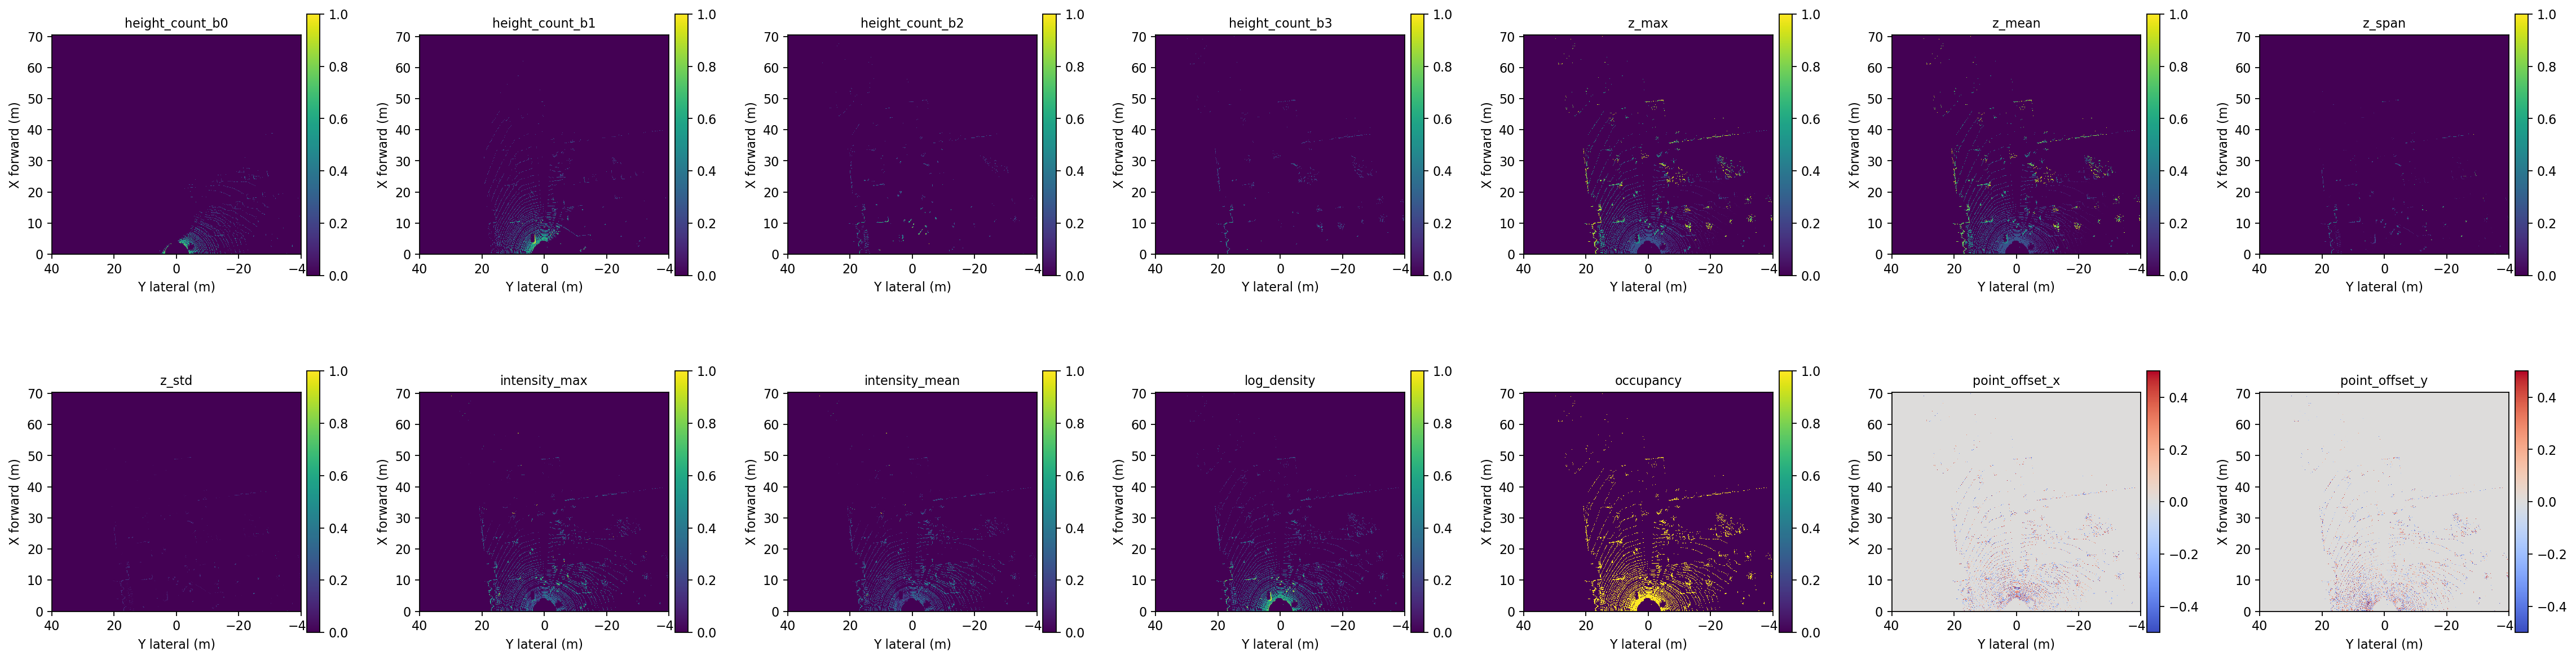
\includegraphics[width=.94\textwidth]{hist14_channels.png}
\caption{Supplied Hist14 visualization from the augmented training example 005663. Each panel displays one input statistic; its display normalization is for visualization. This example is not an unaugmented validation prediction.}
\end{figure}

The main 32-channel fusion configuration uses stage shapes $48\times200\times176$, $96\times100\times88$, and $128\times50\times44$. A single $7\times7$ kernel at those strides spans 2.8, 5.6, and 11.2 m in the input grid, respectively; these values are not the full network receptive field. The focal context bottleneck is 64 with dilations $(1,2,3)$. SimAM uses $\lambda=10^{-4}$ and a learned residual scale initialized to $10^{-3}$. ECA uses a one-dimensional channel convolution of kernel size three and the same residual initialization. The optional detail path downsamples the stride-two stem by a depthwise convolution, projects it to the fusion width, and adds a scaled residual at stride four.

\section{Loss definitions and comparison settings}
\label{sec:loss}
For classification probability $p$ and Gaussian target $Y$, the main focal objective sums $-(1-p)^2\log p$ at $Y=1$ and $-p^2(1-Y)^4\log(1-p)$ at $Y<1$, divided by the number of center peaks when nonzero. If there are no peaks, the negative sum is retained. This is the Gaussian center formulation related to Objects as Points~\cite{zhou2019objects}; the underlying focal principle is credited to Lin et al.~\cite{lin2017focal}. Regression is masked to assigned foreground locations. Baseline uses L1, while OGA uses Smooth-L1 with transition parameter one, plus projection and corner geometry. Log-size decoding is clamped to $[-10,10]$ within the geometric loss, and geometric arithmetic uses FP32 with $\epsilon=10^{-6}$.

OGA's adaptive pool contains classification, center, size, yaw, and geometric loss, with a sixth task when IQA is enabled. Each group has independent adaptive state. Its weights sum to the number of pooled tasks. This constraint bounds relative weights before running-scale normalization and does not fix the total gradient norm. Final3D adds masked Smooth-L1 on $(z_b,\log h)$ after the BEV objective, with coefficient one; the vertical term is not adaptively weighted.

Q100 and the earlier P11 use projection-based Q-OGA quality supervision without a separate IQA branch. The objective uses quality-focal exponent one, soft corner assignment temperature 0.05, and range parameters $\alpha_r=2$, $\gamma_r=1.5$, and $r_{\max}=70.4$ m. Coordinate Smooth-L1 terms are multiplied by range weights. The saved protocol identifies the quality target as \texttt{mgiou}, with zero curriculum warmup; it does not establish an exact rotated-IoU quality experiment. Q-OGA is an implementation comparison influenced by quality focal learning~\cite{li2020gfl}, with several simultaneous objective changes. In the matched O100/Q100 pair, only the objective name differs in the supplied configurations. Both use SimAM and complete 100 epochs with eight learning-rate warmup epochs; P11 instead completes 50 epochs without local attention.

\begin{figure}[htbp]
\centering\includegraphics[width=.98\textwidth]{oga.pdf}
\caption{Supplied schematic of the oriented geometry training package. The projection component follows the multi-axis principle of MGIoU~\cite{le2026mgiou}; the accompanying corner objective and bounded task weighting are described in the main text. The diagram is a conceptual summary, with equations and saved configurations defining the implementation.}
\end{figure}

\section{Evaluation and evidence provenance}
\label{sec:provenance}
KITTI~\cite{geiger2012kitti} training and validation manifests contain 3,712 and 3,769 unique frame IDs with no frame overlap. The validation file SHA-256 is \texttt{2f76fc0f69b5d9786f008694274baaa49d878ba076b96529c488939fd83564c0}. The main ablations use the local loader-aligned BEV R40 implementation. This metric restricts original labels to the loader center crop and applies its difficulty and neighboring-class ignore rules. It is not substituted for full-frame reference AP. Detection score threshold is 0.05, suppression threshold is 0.1, and the global cap is 500 after classwise BEV suppression. With IQA, the scoring exponent is 0.5.

The reference source is OpenPCDet revision \texttt{233f849829b6ac19afb8af8837a0246890908755}, directory \path{pcdet/datasets/kitti/kitti_object_eval_python}~\cite{openpcdet}. The saved report verifies unchanged evaluator and overlap sources and real compatible Numba CUDA execution. It retains metric-specific neighboring-class and DontCare behavior. Predictions use all eight camera-coordinate corners, clipping cuboid edges at camera depth 0.1 m before clipping the projected rectangle to the actual image. The orientation representation is $\pi$-symmetric, so AOS is disabled. The epoch-70 checkpoint SHA-256 is \texttt{1d0e0cd11c27229942e31a3424c905e896f29d52f2f209481ac8eeb60088ff55}. The Final3D config digest is \texttt{404fbd003caadb2e98a876ff993a31e01822d6226e9f3c4d6cf8351d4127e036}. Exact source digests and full reports are supplied in the research directory.

\subsection*{Recovery of training-time configurations}
All 21 original archived BEV configuration files contain a post-run \texttt{header\_architecture=shared} field. Their hashes therefore differ from the training-time config hashes in \texttt{run.json}. Removing this single field and serializing with the original formatting reproduces every recorded training hash exactly. Serialized checkpoint parameter names show independent branch convolutions, consistent with the saved parameter counts and the original omitted-key behavior. The manuscript package preserves the unmodified supplied configs in \texttt{research/configs/as\_provided/}, the recovered training configs in \texttt{research/configs/}, and an audit of hashes and checkpoint parameter names in \texttt{configuration\_audit.json}. The new O100 and Q100 configs already match their recorded training digests and require no recovery. Their checkpoint parameter names likewise show independent branch convolutions. No source experiment file is changed. Final3D explicitly uses shared heads and its supplied config already matches the training digest.

\subsection*{Matched retraining provenance}
O100 and Q100 record the same clean source revision, \texttt{2fcd5217c5d14dce1e523126ff59f72266bfd0de}. Their AP-selected and loss-selected reports agree on the validation split, Hist14 semantic digest, and per-frame input asset hashes. Each detector contains 666,769 backbone/neck parameters and 148,975 head parameters; ten train-only criterion parameters are excluded. Both use score threshold 0.05, NMS threshold 0.1, a global cap of 500, and no IQA score multiplication (exponent zero). The original config, run record, 100 epoch records, selection records, and four raw evaluation reports are retained under \path{research/loss_retrain/}. Config and checkpoint identities are checked by SHA-256; the derived comparison and checks are in \path{research/loss_retrain_comparison.json}.

\subsection*{Scope of the assembled evidence}
The manuscript preparation reads 21 original run directories and 41 saved BEV evaluation reports, plus two newly supplied retraining directories with four reports: 23 BEV runs and 45 reports in total. The separately supplied Final3D evaluations and CPU diagnostic are additional evidence. Preparation performs no new detector training, inference, or benchmark execution. Numeric AP and parameter values are checked against raw JSON, which takes precedence over spreadsheet cells that have been interpreted as dates. The paper's figures are either supplied images/vector diagrams or plots computed from these saved values. The complete editable 25-slide PowerPoint is preserved. Slide 21 and its supplied vector counterpart match the P16 BEV architecture; early illustrative slides contain inconsistent labels and are not used as the authoritative model specification.

\section{Full ablations, operating points, and checkpoint selection}
\label{sec:ablation}
Table~\ref{tab:designs} defines the manuscript run labels. B0 and B1 are historical loss-selected runs with unequal budgets. The other 19 original runs complete 50 epochs and use AP-based selection. The new O100/Q100 pair completes 100 epochs and supplies the main direct OGA--Q-OGA comparison; P11 remains an earlier 50-epoch result. P1--P4 hold the central architecture and training recipe fixed while changing the objective and quality head. P4/P14/P15/P16 change the local refinement module. Earlier comparisons have additional configuration or source differences; Table~\ref{tab:limits} states the appropriate interpretation. The originally supplied operating-point CSV uses label B0 for the later S32 baseline; the manuscript consistently reserves B0 for historical MobilePIXOR.

\begin{table}[htbp]
\centering\small
\caption{Run definitions. F and H denote fusion and prediction widths. The main P-series uses Hist14, grouped heads, F32/H32, and the main hybrid sampling recipe.}
\label{tab:designs}
\begin{tabular}{lp{12.1cm}}
\toprule Run & Configuration \\
\midrule
B0 & Historical MobilePIXOR, binary35, 38 completed epochs of 100 configured, loss-selected epoch 30. \\
B1 & Historical MobilePixorNeXt, binary35, 100 epochs, loss-selected epoch 13. \\
E8 / E14 & Rich8 / Hist14 inputs; single head and standard augmentation. \\
G16 & Hist14, grouped prediction heads of width 16, standard augmentation. \\
O24G16 / O32G16 & Simplified hybrid sampling; gated neck F24 / F32, H16. \\
O24G32 & Simplified hybrid sampling; gated neck F24, H32. \\
O32 & Simplified sampler with probability one; ungated F32/H32. \\
H32 & Hybrid sampler, earlier quotas 6/8/10; ungated F32/H32. \\
S32 & Hybrid sampler, quotas 15/10/10; gated F32/H32; baseline loss, no focal context or IQA. \\
RC24 & Hybrid sampler with range-conditioned neck F24/H32. \\
P1 / P2 & Focal context; baseline / OGA loss; no IQA. \\
P3 / P4 & Focal context; baseline / OGA loss; separate IQA. \\
P5 & OGA plus IQA with focal context disabled. \\
P11 & Q-OGA, focal context, no separate IQA. \\
P14 / P15 / P16 & P4 with detail path / ECA / SimAM, respectively. \\
O100 / Q100 & Matched OGA / Q-OGA, focal context, SimAM, independent F32/H32 grouped heads, no IQA; 100 epochs, AP-selected epoch 70. \\
Final3D & Separate 100-epoch shared-head model with vertical branch, OGA, IQA, focal context, and SimAM; reference 3D-selected epoch 70. \\
\bottomrule
\end{tabular}
\end{table}

\begin{table}[htbp]
\centering\scriptsize\setlength{\tabcolsep}{3pt}
\caption{All 23 local BEV R40 run scores (\%), including the new O100/Q100 pair. E/M/H mean Easy/Moderate/Hard; mAP M is the macro-average across the three Moderate class values. O100/Q100 complete 100 epochs; B0/B1 have historical budgets and loss selection; other runs complete 50 epochs.}
\label{tab:allap}
\begin{tabular}{lrrrrrrrrrr}
\toprule
Run & Car E & Car M & Car H & Ped. E & Ped. M & Ped. H & Cyc. E & Cyc. M & Cyc. H & mAP M \\
\midrule
B0 & 81.00 & 75.52 & 71.44 & 31.61 & 28.16 & 25.04 & 28.13 & 20.53 & 19.05 & 41.40 \\
O32 & 69.83 & 73.70 & 73.49 & 52.96 & 47.30 & 43.49 & 72.50 & 59.65 & 57.08 & 60.22 \\
H32 & 89.18 & 83.51 & 81.30 & 63.66 & 56.62 & 51.64 & 79.20 & 64.24 & 61.11 & 68.12 \\
RC24 & 88.97 & 82.87 & 80.50 & 61.44 & 54.46 & 50.18 & 82.36 & 66.02 & 62.44 & 67.79 \\
O24G16 & 88.27 & 82.37 & 80.14 & 62.06 & 55.12 & 50.04 & 81.18 & 62.18 & 59.43 & 66.56 \\
O24G32 & 91.01 & 84.88 & 82.57 & 63.07 & 54.88 & 49.91 & 79.12 & 62.08 & 58.94 & 67.28 \\
S32 & 89.26 & 83.31 & 81.15 & 64.38 & 58.33 & 52.59 & 78.94 & 63.74 & 60.85 & 68.46 \\
O32G16 & 86.26 & 81.07 & 79.23 & 61.43 & 54.70 & 49.81 & 80.35 & 62.97 & 60.25 & 66.25 \\
E14 & 86.72 & 79.97 & 75.56 & 49.50 & 45.36 & 41.41 & 40.34 & 25.10 & 24.06 & 50.14 \\
G16 & 85.27 & 77.54 & 74.32 & 47.54 & 43.04 & 39.72 & 53.64 & 33.30 & 31.23 & 51.30 \\
B1 & 79.77 & 75.24 & 71.39 & 48.21 & 44.36 & 40.52 & 37.27 & 23.20 & 21.77 & 47.60 \\
E8 & 85.74 & 78.35 & 74.78 & 41.86 & 38.48 & 34.97 & 37.93 & 25.29 & 23.14 & 47.37 \\
P1 & 88.57 & 82.97 & 80.69 & 64.87 & 56.99 & 52.15 & 77.66 & 62.17 & 59.07 & 67.38 \\
P2 & 88.24 & 84.09 & 82.90 & 64.56 & 57.93 & 53.28 & 82.02 & 64.88 & 62.14 & 68.97 \\
P3 & 90.22 & 84.13 & 81.42 & 66.43 & 59.45 & 53.99 & 86.24 & 67.34 & 63.97 & 70.31 \\
P4 & 89.61 & 84.87 & 83.42 & 66.67 & 59.63 & 55.00 & 83.55 & 67.24 & 63.96 & 70.58 \\
P5 & 88.65 & 84.10 & 82.69 & 64.61 & 58.31 & 53.74 & 78.93 & 63.76 & 61.05 & 68.72 \\
P11 & 88.91 & 84.89 & 82.82 & 63.77 & 57.15 & 52.85 & 83.13 & 65.56 & 62.38 & 69.20 \\
P14 & 89.03 & 84.30 & 82.72 & 66.75 & 59.70 & 54.95 & 81.53 & 66.04 & 63.28 & 70.01 \\
P15 & 88.01 & 83.64 & 82.40 & 66.11 & 59.77 & 55.10 & 83.92 & 66.29 & 62.97 & 69.90 \\
P16 & 89.75 & 84.72 & 83.40 & 67.80 & 60.66 & 55.86 & 84.37 & 67.60 & 64.40 & 70.99 \\
O100 & 89.34 & 84.88 & 83.05 & 63.13 & 57.06 & 52.35 & 83.24 & 67.13 & 63.83 & 69.69 \\
Q100 & 88.18 & 84.77 & 83.32 & 66.48 & 61.27 & 55.76 & 82.90 & 65.51 & 62.21 & 70.52 \\
\bottomrule
\end{tabular}

\end{table}

\begin{table}[htbp]
\centering\small\setlength{\tabcolsep}{5pt}
\caption{Saved model size and runtime for all 23 BEV runs, with their individual budgets. Selected is the evaluated checkpoint epoch. Timing is FP32 on an L4, and pipeline denotes offline input-to-detections. Final3D has 797,382 parameters and no saved stage latency.}
\label{tab:allruntime}
\begin{tabular}{lrrrrrr}
\toprule
Run & Epochs & Selected & Parameters & Model ms & Pipeline ms & Pipeline Hz \\
\midrule
B0 & 38 & 30 & 597,817 & 11.050 & 85.923 & 11.64 \\
O32 & 50 & 50 & 789,823 & 6.705 & 65.789 & 15.20 \\
H32 & 50 & 50 & 789,823 & 6.719 & 45.294 & 22.08 \\
RC24 & 50 & 50 & 785,031 & 7.250 & 45.070 & 22.19 \\
O24G16 & 50 & 50 & 669,551 & 7.105 & 45.436 & 22.01 \\
O24G32 & 50 & 50 & 784,383 & 6.877 & 47.963 & 20.85 \\
S32 & 50 & 50 & 790,623 & 6.937 & 45.519 & 21.97 \\
O32G16 & 50 & 50 & 674,639 & 7.449 & 47.943 & 20.86 \\
E14 & 50 & 30 & 650,041 & 5.917 & 77.391 & 12.92 \\
G16 & 50 & 30 & 668,831 & 6.916 & 34.906 & 28.65 \\
B1 & 100 & 13 & 641,977 & 5.883 & 80.797 & 12.38 \\
E8 & 50 & 20 & 648,313 & 6.060 & 40.667 & 24.59 \\
P1 & 50 & 50 & 815,743 & 7.772 & 46.923 & 21.31 \\
P2 & 50 & 50 & 815,743 & 7.827 & 56.380 & 17.74 \\
P3 & 50 & 50 & 852,929 & 8.260 & 45.503 & 21.98 \\
P4 & 50 & 50 & 852,929 & 8.186 & 53.277 & 18.77 \\
P5 & 50 & 50 & 827,809 & 7.813 & 58.588 & 17.07 \\
P11 & 50 & 40 & 815,743 & 7.464 & 43.162 & 23.17 \\
P14 & 50 & 50 & 854,401 & 8.243 & 53.124 & 18.82 \\
P15 & 50 & 50 & 852,933 & 8.510 & 57.862 & 17.28 \\
P16 & 50 & 50 & 852,930 & 8.554 & 56.828 & 17.60 \\
O100 & 100 & 70 & 815,744 & 7.885 & 47.318 & 21.13 \\
Q100 & 100 & 70 & 815,744 & 7.929 & 42.097 & 23.75 \\
\bottomrule
\end{tabular}

\end{table}

\begin{table}[htbp]
\centering\small
\caption{Interpretation of selected comparisons. Differences are observed Moderate local BEV mAP in percentage points for seed 42.}
\label{tab:limits}
\begin{tabular}{lrp{10.4cm}}
\toprule Comparison & $\Delta$ & Interpretation \\
\midrule
E8 $\to$ E14 & +2.77 & Encoding changes alongside source changes; not a clean encoding-only effect. \\
E14 $\to$ G16 & +1.15 & Grouping also accompanies encoding/source and validation-batch differences. \\
O24G16 $\to$ O24G32 & +0.72 & Prediction width increases, with 114,832 more parameters. \\
O24G16 $\to$ O32G16 & $-0.31$ & Wider fusion does not improve this H16 configuration. \\
O32 $\to$ H32 & +7.91 & Sampling probability, quotas, attempts, flags, and batching also change. \\
H32 $\to$ S32 & +0.34 & Gating changes with sampling quotas and validation batching. \\
P1 $\to$ P2 & +1.59 & Complete OGA objective package, without IQA. \\
P3 $\to$ P4 & +0.27 & Complete OGA objective package, with IQA. \\
P4 $\to$ P16 & +0.41 & Residual SimAM comparison in the main configuration. \\
O100 $\to$ Q100 & +0.82 & Matched 100-epoch objective package comparison without IQA; the config differs only in the loss name. \\
P16 $\to$ Final3D & -- & Head topology, vertical outputs, 50/100-epoch budget, selection metric, and evaluator differ. \\
\bottomrule
\end{tabular}
\end{table}

\begin{table}[htbp]
\centering\small
\caption{AP-selected versus loss-selected local BEV checkpoints. AP score and Loss score are Moderate mAP (\%); the difference is AP minus loss in percentage points. O100/Q100 complete 100 epochs; other rows complete 50. Four decimal places in the difference retain O100's small off-grid advantage for loss selection.}
\label{tab:checkpoint}
\begin{tabular}{lrrrrr}
\toprule
Run & AP ep. & AP score & Loss ep. & Loss score & $\Delta$ pp \\
\midrule
S32 & 50 & 68.46 & 42 & 67.89 & +0.5670 \\
P4 & 50 & 70.58 & 25 & 68.92 & +1.6568 \\
P11 & 40 & 69.20 & 34 & 69.15 & +0.0461 \\
P16 & 50 & 70.99 & 28 & 69.83 & +1.1667 \\
RC24 & 50 & 67.79 & 33 & 68.26 & -0.4725 \\
O100 & 70 & 69.69 & 45 & 69.69 & -0.0008 \\
Q100 & 70 & 70.52 & 44 & 69.80 & +0.7190 \\
\bottomrule
\end{tabular}

\end{table}

The primary O100 and Q100 checkpoints are both epoch 70, selected among the ten scheduled AP evaluations. Their minimum-loss checkpoints are epochs 45 and 44, with objective values 0.988347 and 0.993990, respectively. Those checkpoints score 69.690913\% and 69.796116\% Moderate mAP, reducing the Q-OGA advantage to 0.105203 pp. The OGA loss-selected checkpoint exceeds its AP-selected checkpoint by only 0.000801 pp and was outside the ten-epoch AP schedule. It is retained as a sensitivity result rather than substituted into the primary comparison. The objectives have different definitions and weighting, so their raw numerical minima do not rank detection performance.

The shared-versus-independent worksheet includes prospective architectural parameter re-counts. Those rows do not imply trained accuracy or measured speed for every proposed head. Final3D supplies one actually trained shared-head configuration. Its detector count excludes twelve train-only criterion parameters. The recorded per-group head counts are 65,290 for Car and 65,323 for Pedestrian/Cyclist.

\begin{table}[htbp]
\centering\small
\caption{Operating points at score threshold 0.05 under the local BEV protocol. Micro recall pools the 10,157 Moderate ground-truth objects. O100/Q100 complete 100 epochs without IQA; the preceding rows complete 50 epochs. These are not equal-recall comparisons; pipeline rate is from saved offline measurements.}
\label{tab:operating}
\begin{tabular}{lrrrrr}
\toprule
Run & TP & FP & Recall (\%) & FP/frame & Pipeline Hz \\
\midrule
P2 & 9,047 & 150,412 & 89.07 & 39.91 & 17.74 \\
P3 & 9,004 & 96,714 & 88.65 & 25.66 & 21.98 \\
P4 & 9,081 & 140,340 & 89.41 & 37.24 & 18.77 \\
P11 & 9,066 & 88,206 & 89.26 & 23.40 & 23.17 \\
P16 & 9,112 & 149,111 & 89.71 & 39.56 & 17.60 \\
O100 & 9,089 & 118,795 & 89.49 & 31.52 & 21.13 \\
Q100 & 9,108 & 77,704 & 89.67 & 20.62 & 23.75 \\
\bottomrule
\end{tabular}

\end{table}

\begin{table}[htbp]
\centering\small
\caption{Saved scheduled local BEV R40 Moderate mAP (\%) for the matched 100-epoch pair. Both use seed 42, SimAM, no separate IQA, and the same split and decoder. Epoch 70 is the maximum scheduled score for each objective.}
\label{tab:retraincurve}
\begin{tabular}{rrr}
\toprule
Epoch & OGA mAP & Q-OGA mAP \\
\midrule
10 & 48.40 & 52.41 \\
20 & 63.84 & 60.39 \\
30 & 65.60 & 68.84 \\
40 & 69.43 & 70.33 \\
50 & 67.28 & 68.29 \\
60 & 67.38 & 67.98 \\
70 & 69.69 & 70.52 \\
80 & 68.17 & 69.50 \\
90 & 69.25 & 69.86 \\
100 & 68.79 & 70.32 \\
\bottomrule
\end{tabular}

\end{table}

\begin{figure}[htbp]
\centering\includegraphics[width=.98\textwidth]{loss_retrain_objectives.pdf}
\caption{Recorded training and validation objectives for the supplied 100-epoch O100/Q100 runs, on logarithmic axes. Every epoch is shown, including the large initial values. Each curve describes convergence under its own objective definition and adaptive weighting. Raw OGA and Q-OGA loss values are not directly comparable measures of detector accuracy; Table~\ref{tab:retraincurve} gives their common AP metric. Learning-rate warmup lasts eight epochs; the Q-OGA quality curriculum is disabled.}
\label{fig:retrainobjectives}
\end{figure}

\clearpage
\section{Qualitative artifacts and conditional vertical analysis}
\label{sec:demo}
The supplied demonstration checkpoint is P4, selected at epoch 50. Frame 004338 belongs to validation and frame 005663 to training. The augmented pipeline example uses frame 005663, random seed two, and 17 inserted ground-truth objects drawn from training donors. It illustrates data processing rather than detector accuracy on an unseen frame. Feature maps depict root-mean-square activations, classification maps show sigmoid scores, and Gaussian supervision maps show targets; they are distinct quantities.

\begin{figure}[htbp]
\centering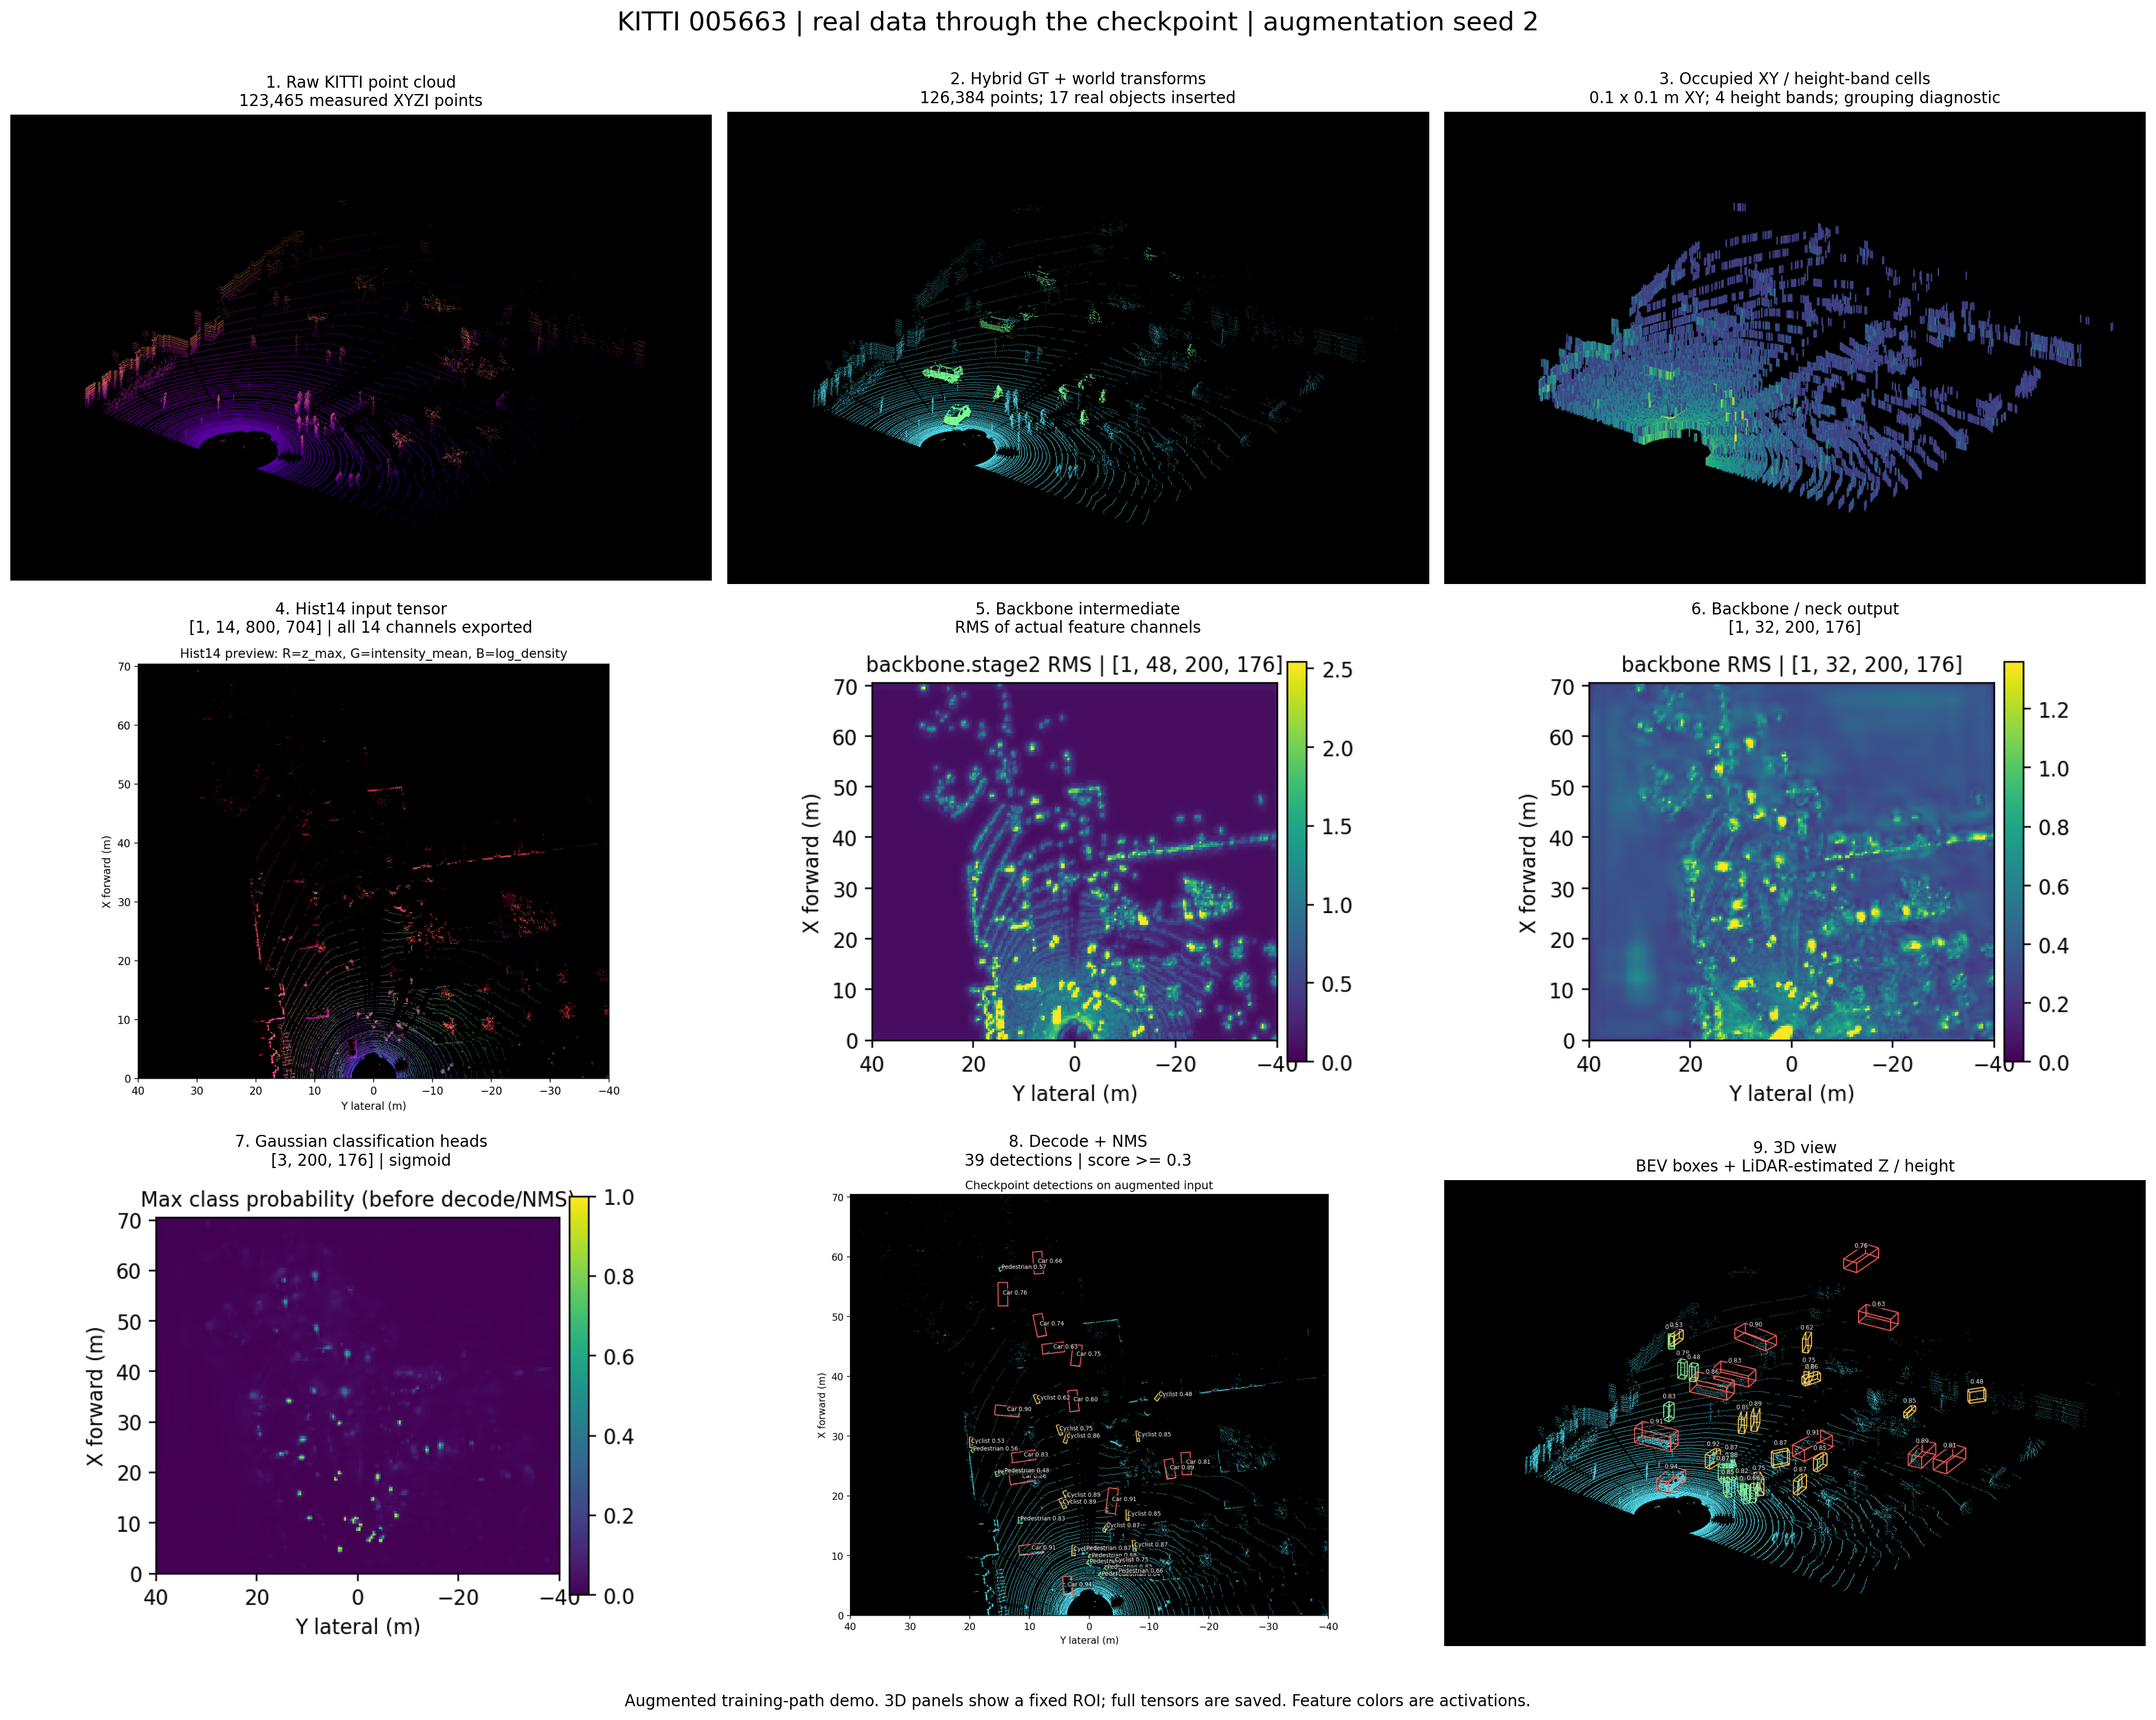
\includegraphics[width=.94\textwidth]{training_pipeline.png}
\caption{Supplied augmented training example 005663, with point-cloud augmentation, Hist14 encoding, intermediate feature visualizations, heatmaps, decoded footprints, and a LiDAR-derived cuboid display. The cuboid vertical extent is estimated from points rather than predicted by Final3D. The panels are a pipeline illustration, not an AP experiment.}
\end{figure}

\begin{figure}[htbp]
\centering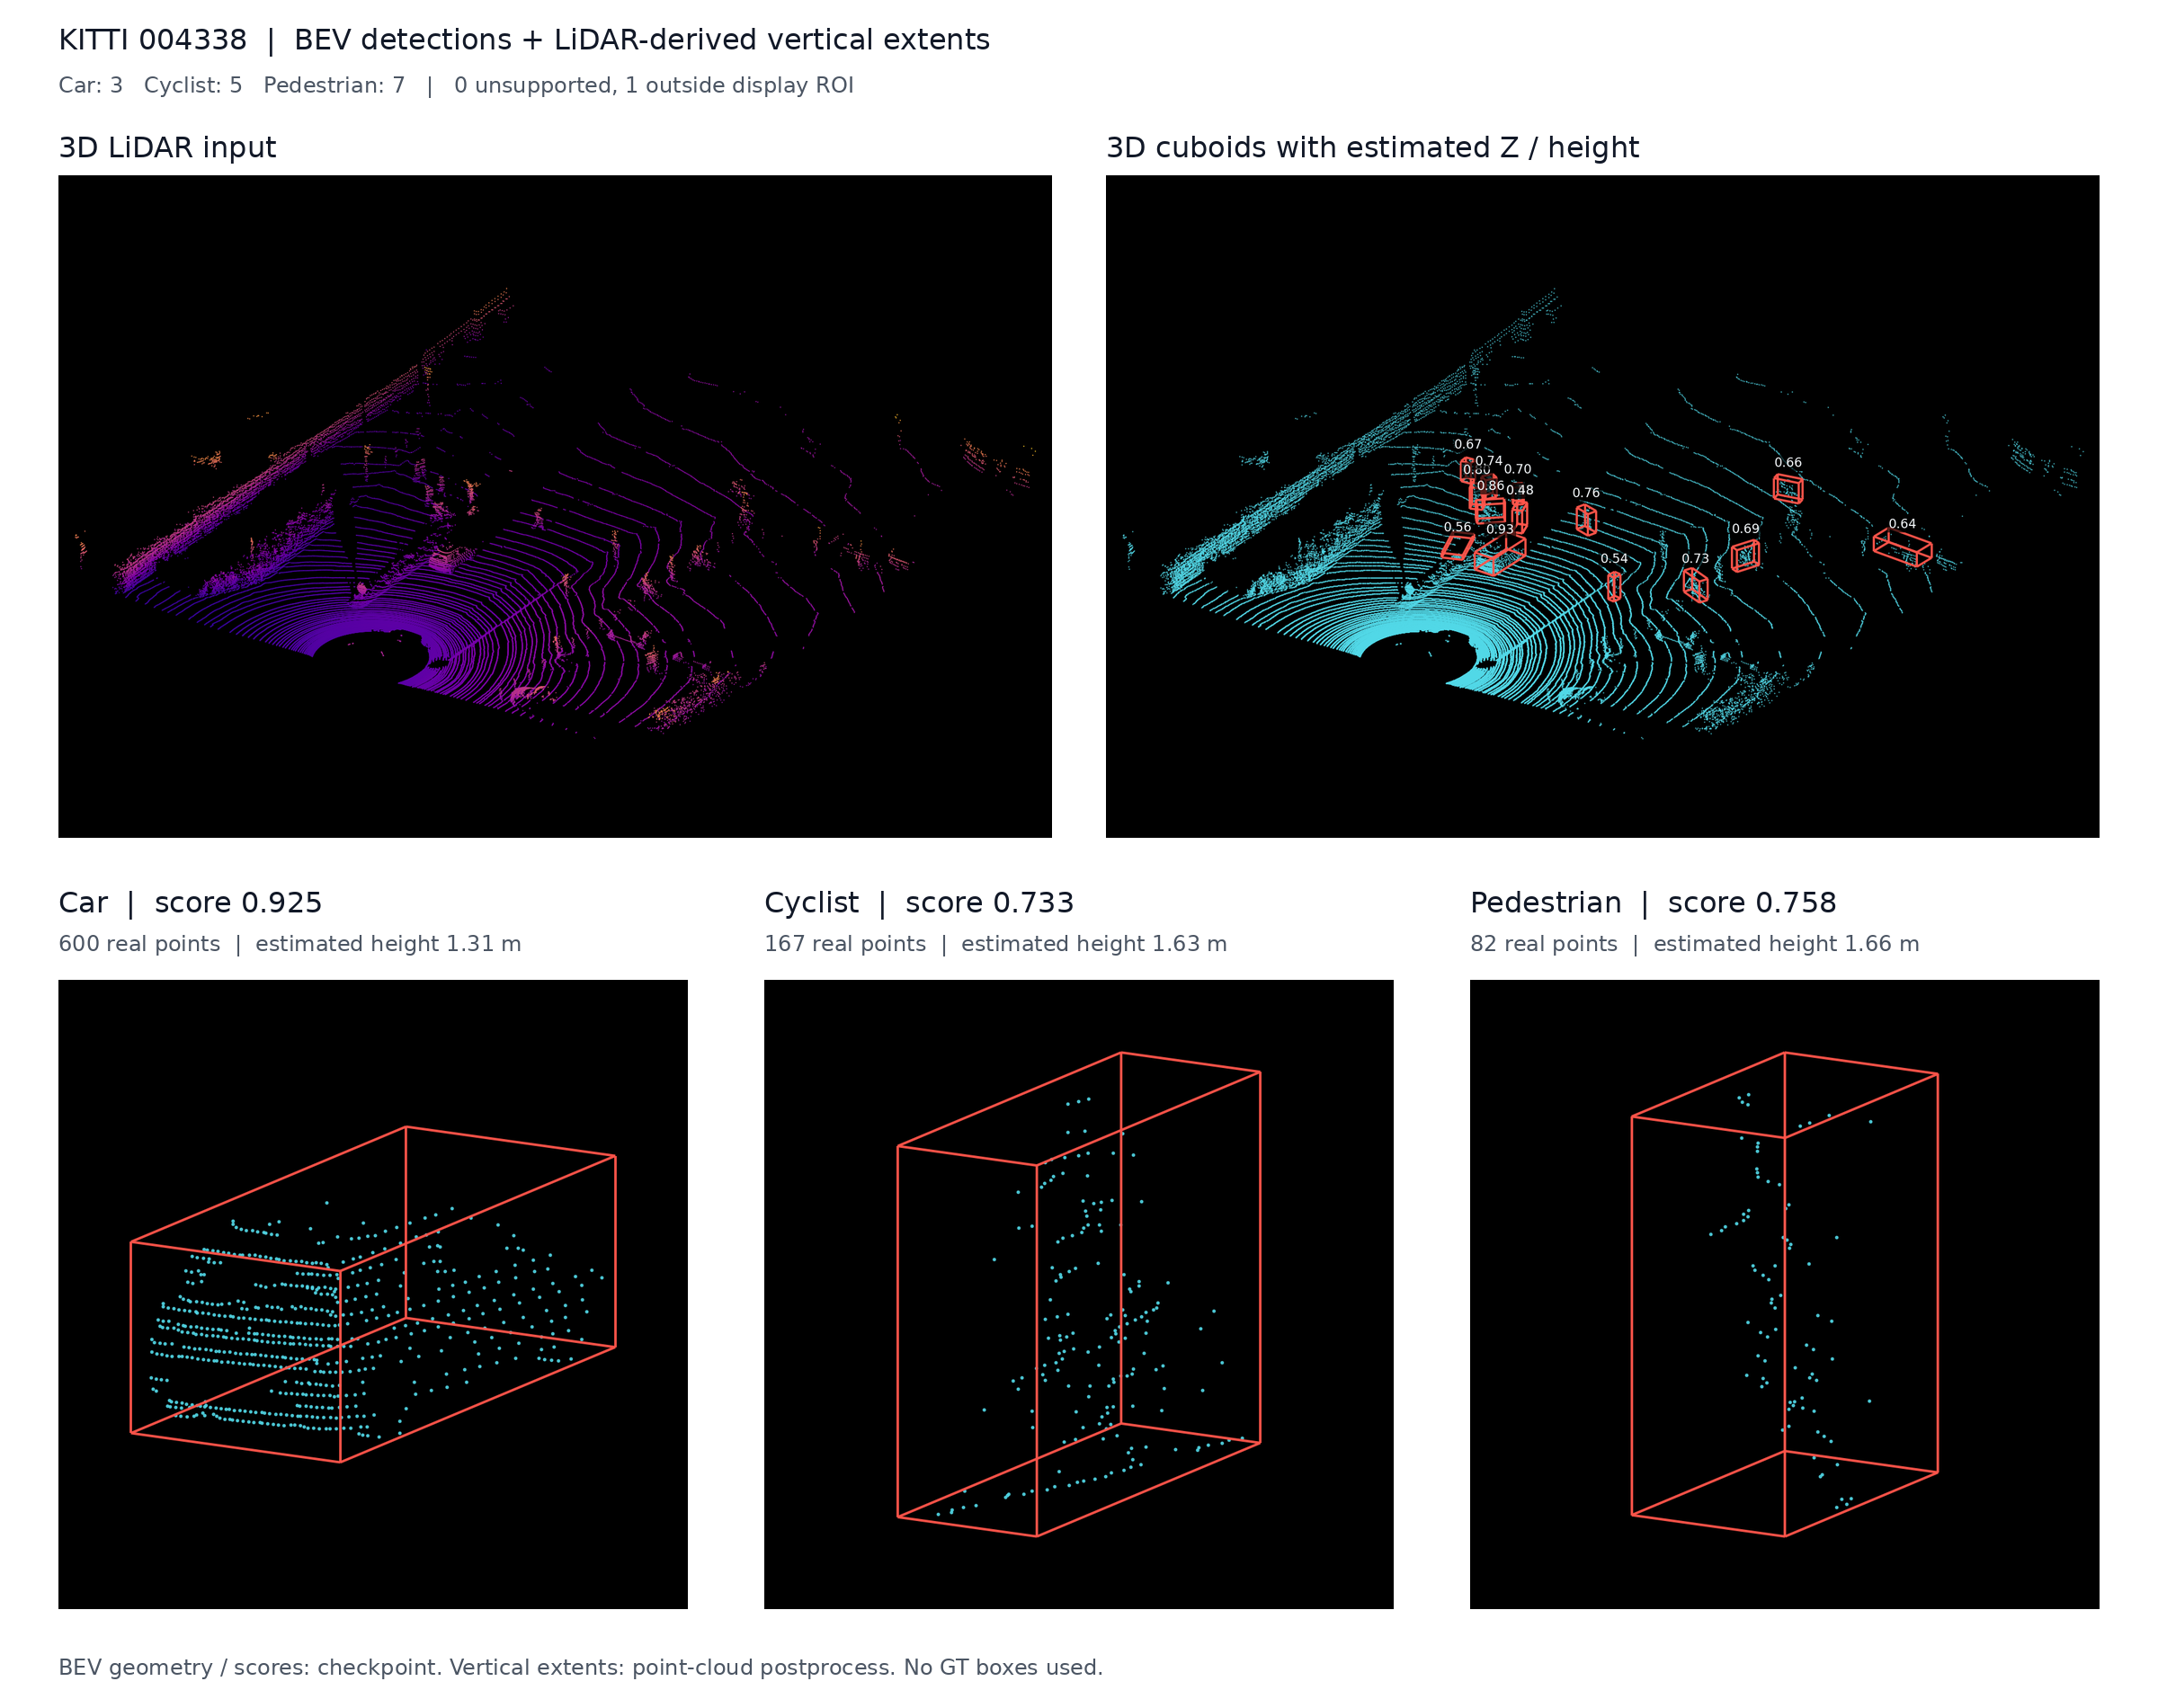
\includegraphics[width=.85\textwidth]{validation_lift.png}
\caption{Supplied validation frame 004338 with P4 BEV footprints lifted to cuboids using LiDAR-estimated vertical extent. This image does not demonstrate the separately trained vertical branch.}
\end{figure}

The supplied videos show 174 consecutive validation frames corresponding to raw sequence \path{2011_09_26_drive_0014_sync}, raw frame indices 77--250, from the KITTI raw data~\cite{geiger2013raw}. The camera is used only for display. The 10-frame/s playback rate yields a 17.4-second clip and is not a measured inference rate. The contact sheet in Fig.~\ref{fig:sequence} provides temporal examples without establishing tracking accuracy.

\begin{figure}[htbp]
\centering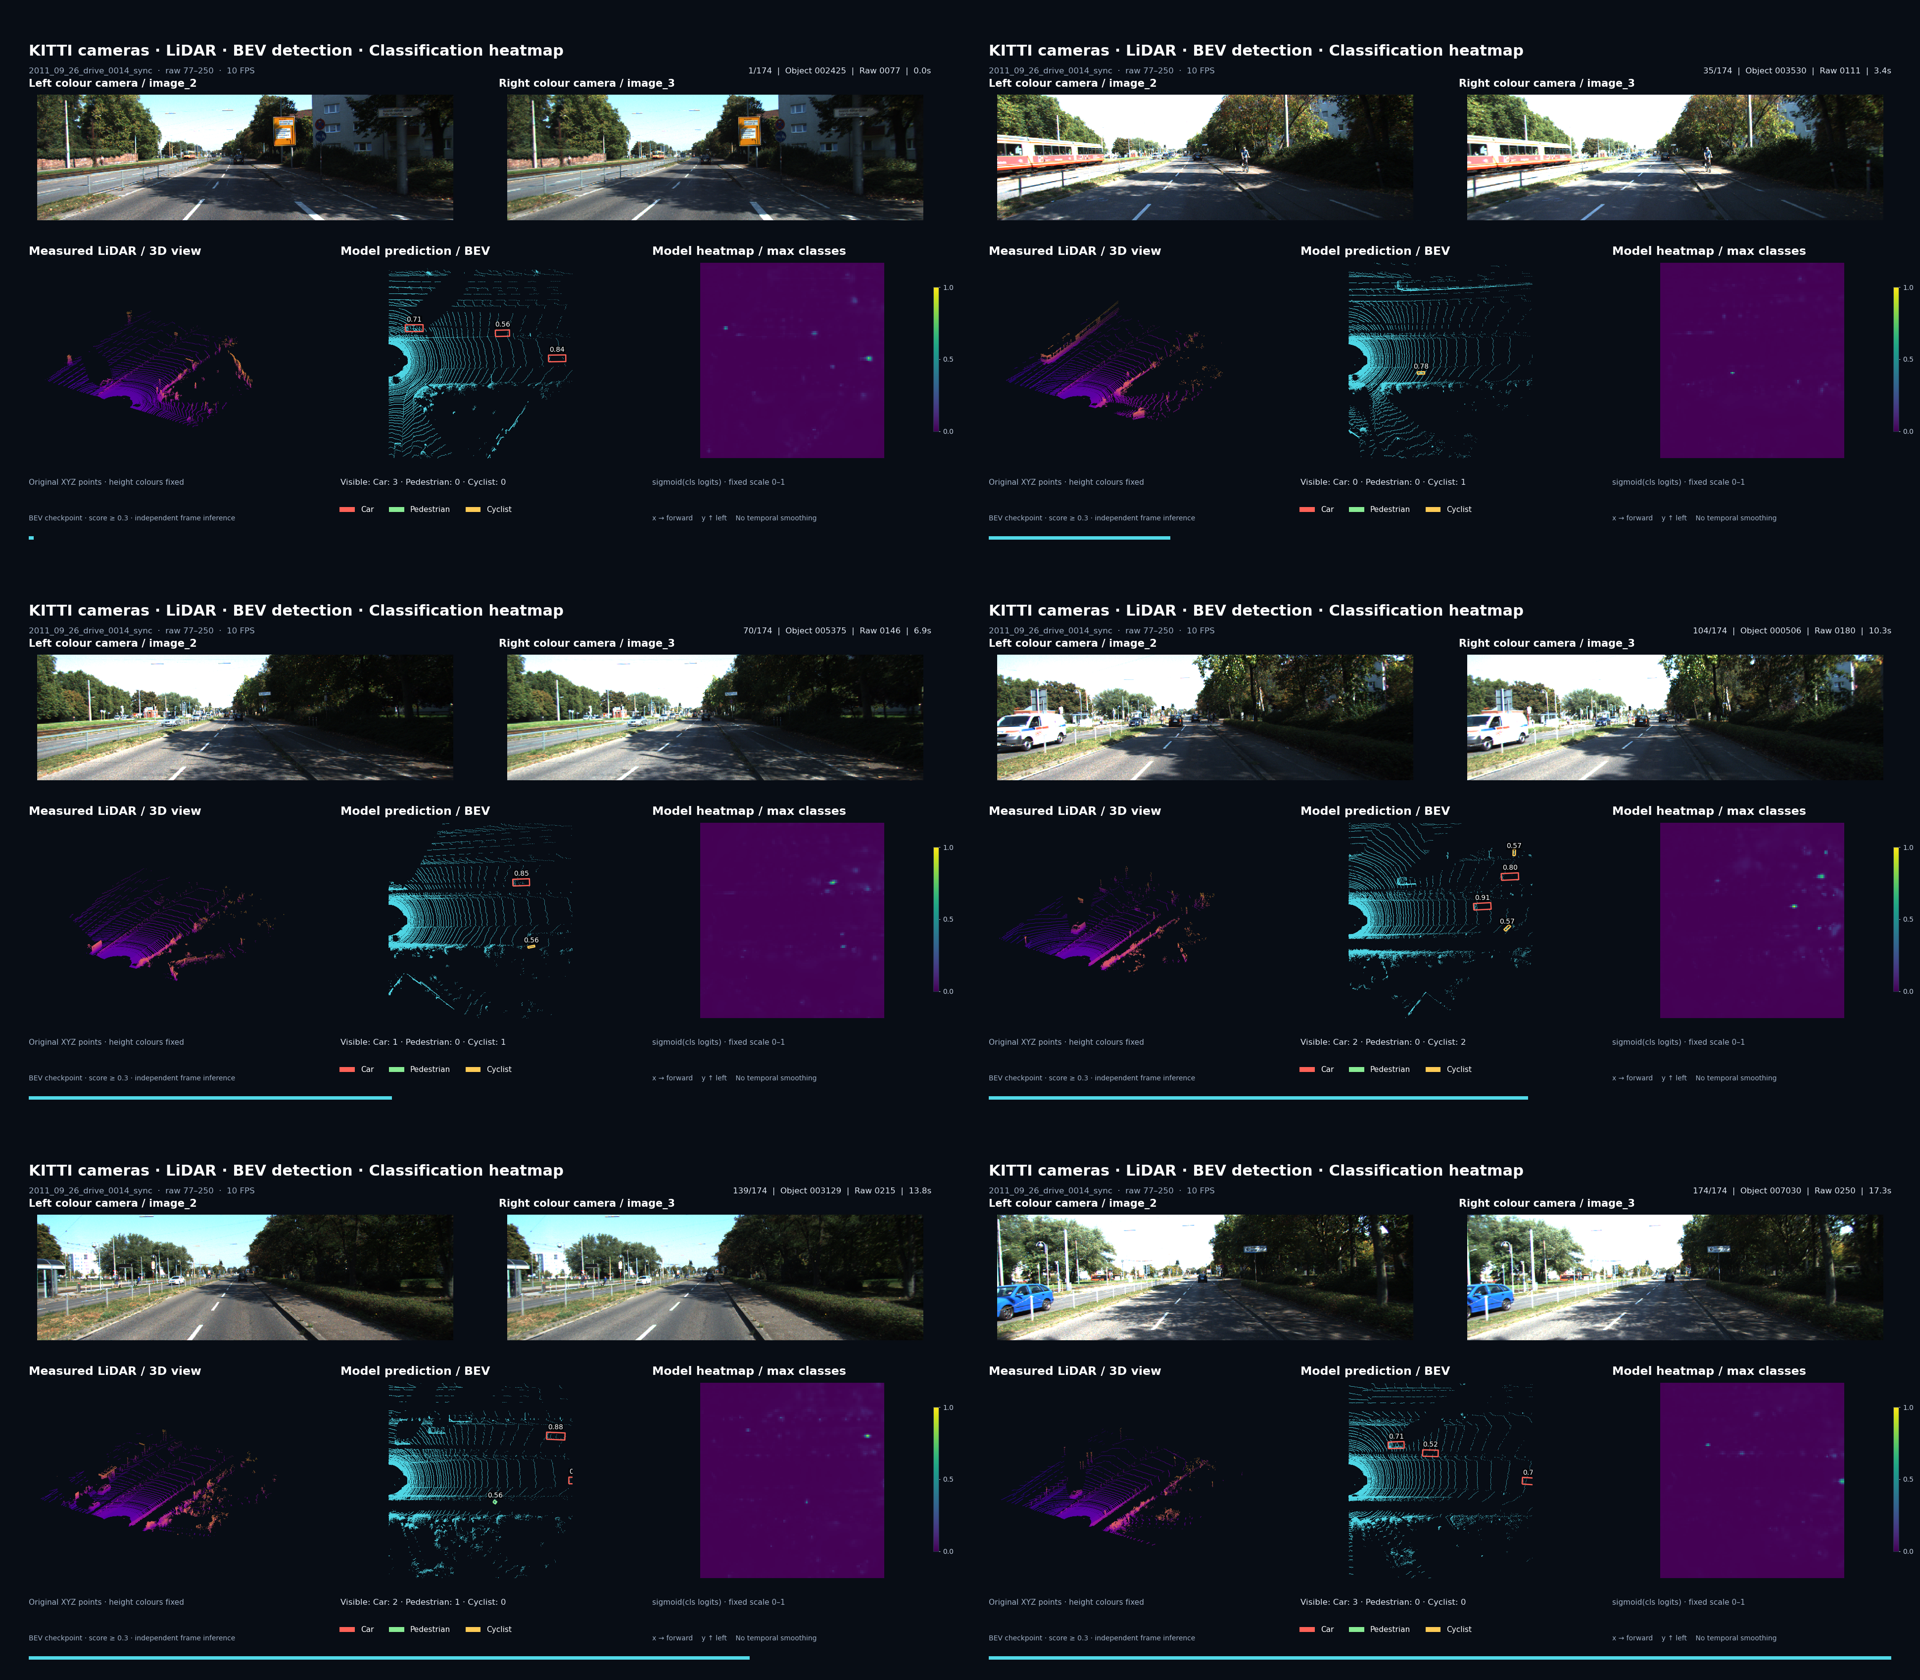
\includegraphics[width=.98\textwidth]{sequence.png}
\caption{Supplied contact sheet from the camera/LiDAR/BEV/heatmap sequence. It uses the P4 BEV checkpoint and consecutive validation frames. No tracking metric or trained Final3D result is inferred from this visualization.}
\label{fig:sequence}
\end{figure}

The existing CPU geometric diagnostic uses the same epoch-70 checkpoint digest as the GPU reference evaluation and verifies 3,769 scan, label, and calibration inputs against stored hashes. It obtains 107,194 projected detections, compared with 107,073 in the saved GPU report. Associations are fixed before oracle substitution and omit metric-specific ignored neighbors and DontCare treatment. Therefore, conditional pass fractions, objectwise errors, and reference AP remain distinct measurements.

\begin{table}[htbp]
\centering\small
\caption{Conditional 3D IoU threshold passes on fixed CPU BEV pairs, at score exponent 0.5. Oracle location means camera-coordinate bottom vertical position. The threshold is 0.7 for Car and 0.5 for Pedestrian/Cyclist. No oracle AP is computed.}
\begin{tabular}{lrrrrr}
\toprule Class & BEV pairs & Predicted & Oracle location & Oracle height & Both oracles \\
\midrule
Car & 7,130 & 5,743 & 6,791 & 5,873 & 7,130 \\
Pedestrian & 1,342 & 1,193 & 1,297 & 1,210 & 1,342 \\
Cyclist & 448 & 412 & 441 & 410 & 448 \\
\bottomrule
\end{tabular}
\end{table}

For Cars, replacing height alone recovers 391 failing pairs but causes 261 previously passing pairs to fail; its net improvement is only 130. This illustrates coupled location and height errors. The Car bottom-height absolute error is 7.28 cm at 0--20 m, 8.86 cm at 20--40 m, and 12.38 cm beyond 40 m, among 2,739, 3,571, and 820 fixed BEV matches. Corresponding 3D pass fractions are 91.46\%, 78.44\%, and 53.29\%. These conditional samples are not representative of objects missed in BEV. Scores, original projected image boxes, and associations are deliberately frozen in the oracle analysis, so a fresh reference evaluation would be needed to quantify changes in detection AP.

\clearpage
\bibliographystyle{IEEEtran}
\bibliography{references}
\end{document}
